\chapter{Access to the VSC Cloud}

The Globus platform enables developers to provide robust file transfer, sharing and search capabilities within their own research data applications and services, while leveraging advanced identity management, single sign-on, and authorization capabilities.

\section{Log in with an existing identity}\label{login}

Visit \href{https://www.globus.org}{www.globus.org} and click \emph{Login} at the top of the page. On the Globus login page, choose an organization you are already registered with, such as your school or your employer.

\begin{center}
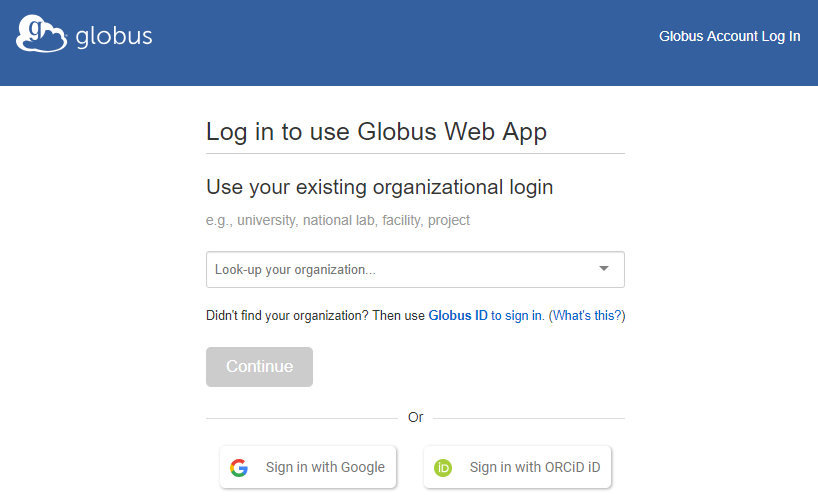
\includegraphics[width=0.5\textwidth]{img/access-login-screen.png}
\end{center}

When you find it, click \emph{Continue}. If you cannot find your organization in the list, you can use Google, ORCID, or Globus ID, all three of which allow you to create new accounts if you do not already have one.

You will be redirected to your organization's login page. Use your credentials for that organization to login.

Some organizations will ask for your permission to release your account information to Globus.

Once you have logged in with your organization, Globus will ask if you would like to link to an existing account. If this is your first time logging in to Globus, click \emph{Continue}. If you have already used another account with Globus, you can choose \emph{Link to an existing account}.

You may be prompted to provide additional information such as your organization and whether or not Globus will be used for commercial purposes. Complete the form and click \emph{Continue}.

Finally, you need to give Globus permission to use your identity to access information and perform actions (like file transfers) on your behalf.

\begin{center}
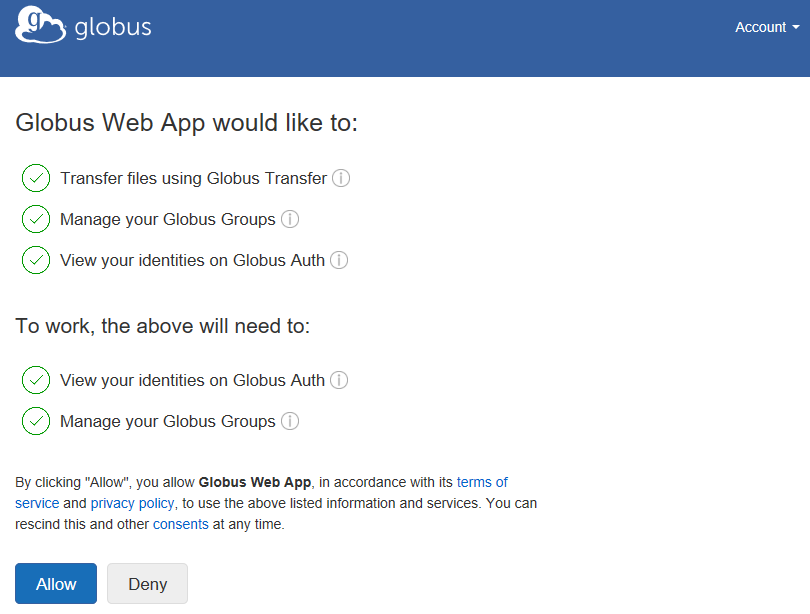
\includegraphics[width=0.5\textwidth]{img/access-first-time-login-permissions.png}
\end{center}

%%% Local Variables:
%%% mode: latex
%%% TeX-master: "intro-Globus"
%%% End:
